\documentclass[10pt]{article}
\usepackage[margin=20mm]{geometry}
\usepackage{graphicx,booktabs,amsmath}
\usepackage[hidelinks]{hyperref}
\title{Supplementary diagnostics: local-volatility calibration}
\author{Anonymous submission}
\date{}
\begin{document}\maketitle
This supplement is generated from executed experiments. Profile: paper.
Smoke and pilot outputs are validation/exploration, not final study evidence.
Every figure has a same-name JSON source record. Full metrics, unsuccessful
optimisation runs, failed baseline calls, and invalid implied-volatility counts
are retained in the accompanying CSV/JSON files.
\begin{figure}[htbp]\centering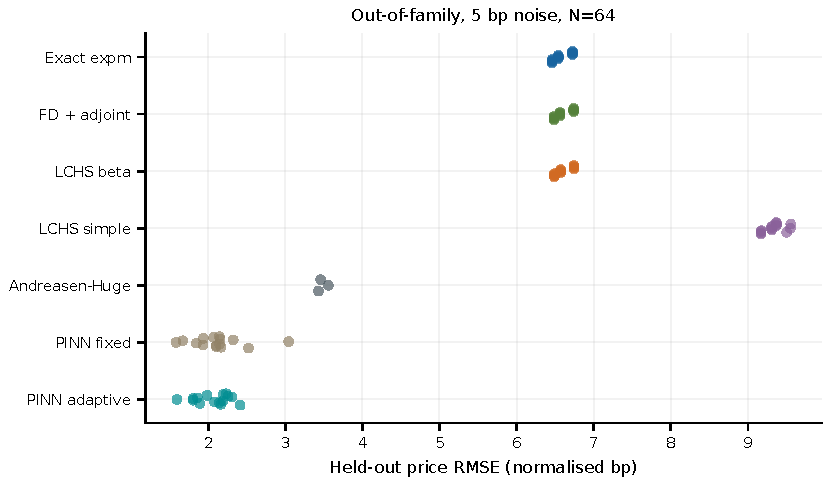
\includegraphics[width=.92\linewidth]{figures/benchmark_variability.pdf}\caption{All executed initialisations, out-of-family noisy case.}\end{figure}
\begin{figure}[htbp]\centering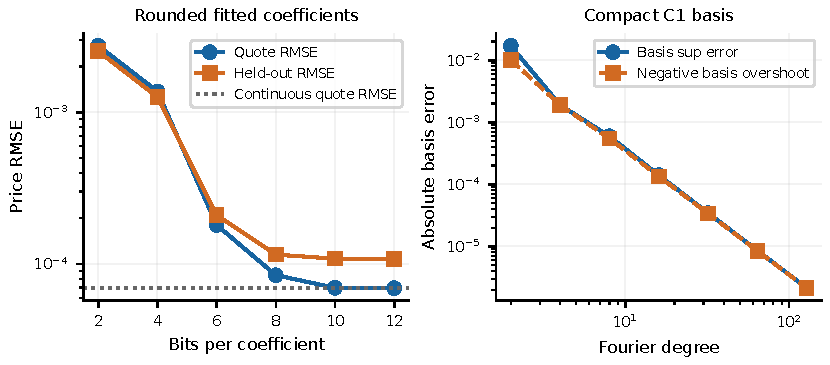
\includegraphics[width=.92\linewidth]{figures/precision_basis.pdf}\caption{Coefficient rounding and global Fourier approximation.}\end{figure}
\begin{figure}[htbp]\centering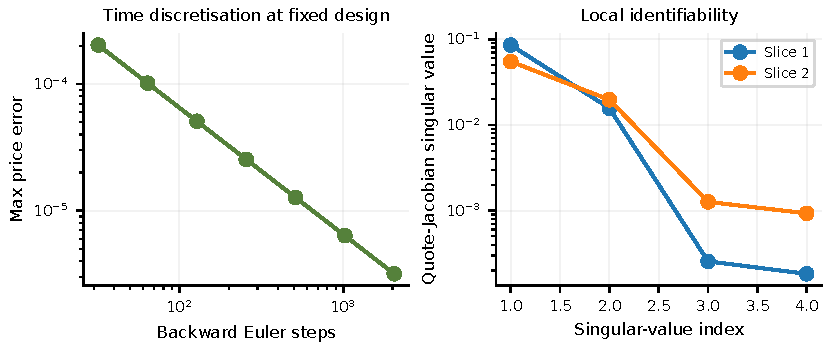
\includegraphics[width=.92\linewidth]{figures/fd_identifiability.pdf}\caption{Time-discretisation and local identifiability diagnostics.}\end{figure}
\begin{figure}[htbp]\centering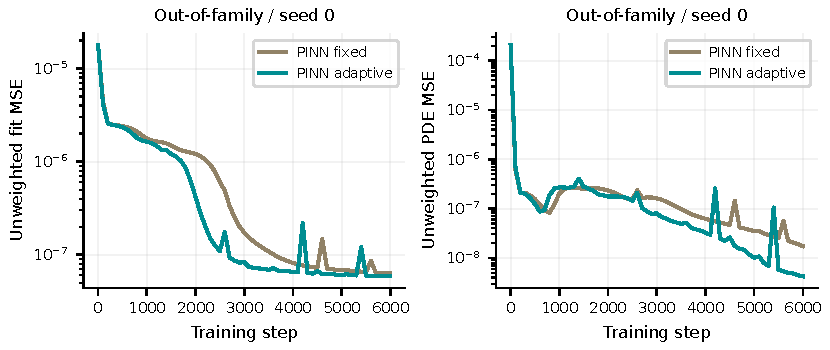
\includegraphics[width=.92\linewidth]{figures/pinn_losses.pdf}\caption{Documented fixed/adaptive PINN comparison.}\end{figure}
\begin{figure}[htbp]\centering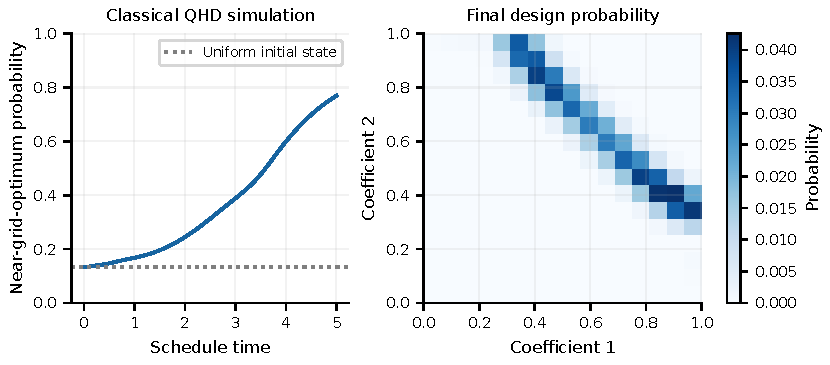
\includegraphics[width=.92\linewidth]{figures/qhd_diagnostics.pdf}\caption{Classically tabulated QHD simulation; see qhd\_refinement.csv.}\end{figure}
\begin{figure}[htbp]\centering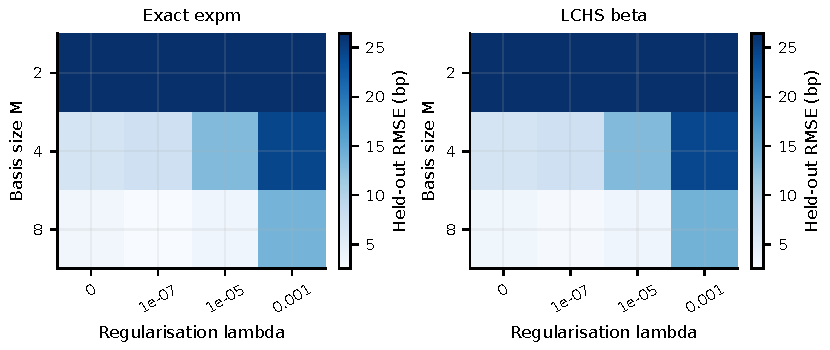
\includegraphics[width=.92\linewidth]{figures/ablation.pdf}\caption{Independent basis-size and regularisation ablation.}\end{figure}
\begin{figure}[htbp]\centering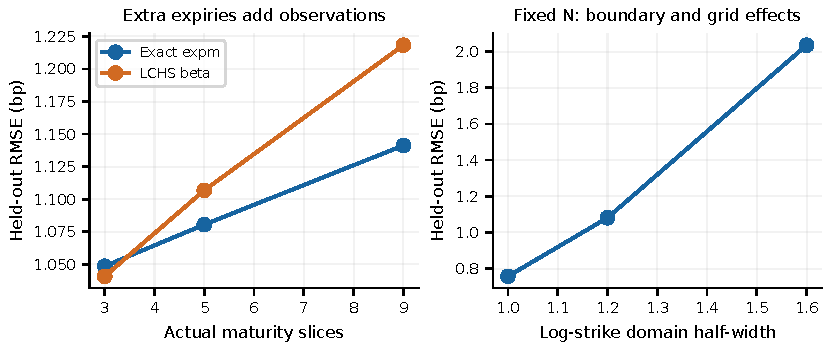
\includegraphics[width=.92\linewidth]{figures/domain_slices.pdf}\caption{Maturity and finite-domain sensitivity, with explicit confounders.}\end{figure}
\end{document}